% Copyright 2007 by Till Tantau
%
% This file may be distributed and/or modified
%
% 1. under the LaTeX Project Public License and/or
% 2. under the GNU Public License.
%
% See the file doc/licenses/LICENSE for more details.


\lecture[18]{Estimating proportions}{lecture-text}

\subtitle{with confidence}

\date{2 April 2015}


\begin{document}

\begin{frame}
  \maketitle
\end{frame}


\begin{frame}{So far we have}
  \begin{enumerate}
    \item analyzed \alert{quantitative} data:
    \item when each observation is a numerical measurement,
    \item using means, standard deviations, ranks, etcetera.
    \item \alert{Categorical data} assigns each observation to a discrete category,
    \item and we analyze the proportions, or counts in each.
  \end{enumerate}
\end{frame}

\begin{frame}\frametitle<presentation>{Outline}
  \tableofcontents
\end{frame}



\section{Estimating the sample proportion}
\subsection{Intuition}

%%%%%%
\begin{frame}{Not so obvious}

    In a random sample of 20 pigeons in Los Angeles,
    we see 5 with brown heads and 15 with grey heads.\\
    \structure{What do you think the true proportion of Los Angeles pigeons with brown heads is?}

    \vspace{2em}

    \pause

    We sample another 80 pigeons, and find \emph{none} with green-polka-dotted heads.\\
    \structure{What do you think the true proportion of Los Angeles pigeons with green-polka-dotted heads is?}

    \vspace{2em}

    \pause

    We know some pigeons have white heads due to interbreeding with escaped domestic birds,
    but \emph{none} of the 100 pigeons we have so far have white heads.\\
    \structure{What do you think the true proportion of Los Angeles pigeons with white heads is?}

    \vspace{1em}
    \pause

    \alert{Is it reasonable} that the true proportion of pigeons with white heads is 10\%?


\end{frame}

%%%%%%
\begin{frame}{Estimates, and uncertainty}

    We have a random sample of observations falling in two categories.

    \vspace{2em}

    We want to
    \begin{enumerate}
        \item Estimate the population frequency.
        \item Evaluate our uncertainty about that estimate.
    \end{enumerate}

    \vspace{2em}

    If you observe \alert{none} of one category, \\
        should you estimate that the population really has none? \\
            \hspace{3em} \structure{Usually not.}  {\small (else, why were you looking?)}

\end{frame}

\subsection{Estimating the population frequency}

%%%%%%
\begin{frame}{The sampling distribution}

    \begin{block}{Central Limit Theorem for Frequencies}
        If $Y$ is the number of observations of type ``A''
        out of a sample of $n$ independent draws
        from a large population with a true frequency $p$ of type ``A'', \\
        then $Y$ is \alert{approximately Normal},
        with mean $np$ and standard deviation $\sqrt{n p (1-p)}$,
        if $n$ is large enough.
    \end{block}

    \vspace{2em}

    This implies that 
    \[ \prob\left( np - 1.96 \sqrt{n p(1-p)} \le Y \le np + 1.96 \sqrt{n p (1-p)} \right) \approx 0.95 , \]
    i.e.\ the number of observed type ``A'' should be about $np$, give or take $2 \sqrt{n p (1-p)}$ or so.

    \vspace{2em}

    \structure{simulation example}

\end{frame}

%%%%%%
\begin{frame}{The standard error for $\hat p$}

    The \alert{sample proportion} of type A is
    the fraction of the sample that is type A:
    \[ \hat p = \frac{y}{n} . \]

    \vspace{2em}

    By the Central Limit Theorem, we know that 
    \[  \hat p \approx p \pm 2 \sqrt{ \frac{ p(1-p) }{ n } } .\]

    \vspace{2em}

    But, we don't actually know the population proportion $p$.

\end{frame}

%%%%%%
\begin{frame}{An estimator for $p$}

    \begin{block}{Wilson's estimator}
        for the population proportion is
        \[ \wt p = \frac{ y+2 }{ n+4 } ,\]
        i.e.\ the frequency in the sample with two imaginary observations of each type added.
    \end{block}

    \vspace{2em}


    \begin{block}{Standard Error}
        for Wilson's estimator is
        \[ \SE_{\wt P} = \sqrt{\frac{\wt p (1-\wt p)}{n+4} } .\]
    \end{block}

    \vspace{1em}
    \structure{Why $+2$?} Problems happen if $\wt p$ is near 0 or 1; Wilson moves the estimate away from these.


\end{frame}

\subsection{Confidence intervals}

%%%%%%
\begin{frame}{Confidence intervals}

    We know that 
    \begin{itemize}
        \item the sampling distribution of Wilson's estimator $\wt P$ is approximately Normal
        \item with standard error $\SE_{\wt P}$,
        \item so a $(1-\alpha)$ confidence interval is $z_{\alpha/2} \SE_{\wt P}$.
    \end{itemize}
    It turns out that this usually does a good job \\
    \alert{even if $n$ is not large.}

    \vspace{2em}

    \begin{block}{A 95\% confidence interval}
        for Wilson's estimator is
        \[ \wt p \pm 1.96 \; \SE_{\wt P} . \]
    \end{block}

    \vspace{2em}

    Check this, \structure{by simulation}.

\end{frame}


%%%%%%
\begin{frame}{Example}

    Out of 169 women with family histories of breast cancer, 27 had mutations in the BRCA1 gene.

    \vspace{2em}

    \alert{Wilson's estimator} gives that around
        \[ \wt p = \frac{27 + 2}{169+4} = .168 \]
    of women with family histories of breast cancer have mutations in BRCA1.

    \vspace{2em}

    The \alert{standard error} of this estimate is
    \[ \SE_{\wt P} = \sqrt{\frac{.168(1-.168)}{169+4}} = .028  \]

    \vspace{2em}

    A \alert{95\% confidence interval} for this proportion is $\wt p \pm 1.96 \times .028$:
    \[ 0.113 < p < 0.223 \]

\end{frame}

%%%%%%
\begin{frame}{From the wild}

    \begin{center}
    \includegraphicscopyright[width=\textwidth]{barn-owl-comparison}{Owl predation in Pennsylvania, Pearson \& Pearson 1947}
    \end{center}

    \vspace{2em}

    Find confidence intervals for some of these percentages.  
    Is there strong evidence that owls catch a higher percentage than traps of 
    \textit{(a)} meadow mice?
    \textit{(b)} Deer mice?
    \textit{(c)} Star-nosed moles?


\end{frame}

%%%%%%
\begin{frame}{Example}

    Eleven newborn babies with respiratory failure were given ECMO.  None died.

    \vspace{2em}

    \alert{Wilson's estimator} of the probability of death is
    \[ \wt p = \frac{0+2}{11+4} = 0.133 \]

    \vspace{2em}

    The \alert{standard error} of this estimate is
    \[ \SE_{\wt P} = \sqrt{\frac{ .133(1-.133) }{ 11+4 }} = .088 \]

    \vspace{2em}

    A \alert{95\% confidence interval} for this proportion is
    \[ -0.039 < \only<2->{ {\color{red} 0 <}} p < 0.305 \]


\end{frame}

%%%%%%
\begin{frame}{One-sided confidence}

    We might often want to \alert{upper bound} the population frequency,\\\
    i.e.\ construct a \structure{one-sided confidence interval}.

    \vspace{2em}

    Since $z_{.05} = 1.645$, 
    a \alert{95\% one-sided CI} is 
        \[ p < \wt p + 1.645 \; \SE_{\wt P} \]

    \vspace{2em}

    In the previous example, this is
        \[ p < 0.278 , \]
    so we are 95\% confident that the true chance of death is less than 27.8\%.


\end{frame}

\subsection{Planning studies}

%%%%%%
\begin{frame}{Pick your SE}

    We want to estimate the population percentage to \alert{1\% accuracy}
    (at 95\% confidence).
    How big a sample should we take?

    \vspace{2em}
    \pause

    \structure{Rephrased:} We want to estimate the population percentage
    with two {\tiny (really, 1.96)} standard errors no larger than 1\%.
    How big a sample should we take?

    \vspace{2em}

    Well,
        \[ 2 \SE_{\wt P} = 2 \sqrt{\frac{\wt p (1-\wt p)}{n+4} } ,\]
        so it \alert<1>{depends on $p$}, \pause but \alert<2->{no matter what $p$ is,}\\
    $\sqrt{p (1-p)} \le 1/2$,
    so
    \[ 2 \SE_{\wt P} \le \sqrt{\frac{1}{(n+4)} } .\]

    \vspace{1em}

    We can guarantee that $2 \SE_{\wt P} \le .01$ if $n \ge 100^2$, \\
    i.e.\ we have at least 10,000 observations.


\end{frame}

%%%%%%
\begin{frame}{Example: polling}

    We want to do a poll to determine whether a state proposition 
    is ahead (above 50\%) or not,
    with 95\% confidence,
    as long it is actually leading (or, behind) by at least 5\%.
    How many people should we poll?
    Assume everyone is decided.
    \pause

    \vspace{2em}

    The 95\% CI is, at worst, $\wt p \pm 1/\sqrt{n+4}$.  \\
    \hspace{3em} We want 0.5 to be \alert{outside} the CI.
    \pause

    \vspace{2em}

    At worst, the true value is $p=0.525$ \\
    \hspace{3em} and it lies at the upper end of the CI.
    \pause

    \vspace{2em}

    So, we want
    \[
    0.525 - 2 \times \frac{1}{\sqrt{n+4}} > 0.5
    \]
    or
    \[
    (n+4) > (2/0.025)^2
    \]
    or $n+4 > 6400$.

\end{frame}

%%%%% %%%%%%% %%%%%%%%
\section{Comparing proportions}

\subsection{More categories}

\begin{frame}{Next: more categories}

  We have so far looked at proportions, i.e.\\
  \structure{counts of a single, dichotomous, categorical variable}.

  \vspace{2em}

  \structure{Next:} more categories.
  
  \vspace{2em}

  Comparing to known proportions, with a hypothesis test.

\end{frame}

\begin{frame}{Example: Hardy--Weinberg}

    Red--green colorblindness is caused by recessive mutations in one of the opsin genes on the X chromosome.
    The frequency in males (only one X) indicates that these mutations are at around $q=8.3\%$ in Europeans.
    % This suggests the frequency in females should be $q^2= 0.69\%$.
    We sample 1000 females and compare frequencies of nonmutants, carriers, and color-blindness to the expected proportions $(1-q)^2$, $2q(1-q)$, and $q^2$:
    \begin{center}
        \begin{tabular}{r|rr}
            & observed counts & expected counts \\
            \hline 
            nonmutant & 850 & 840.9 \\ 
            carrier &  146 & 152.2 \\ 
            colorblind & 4 & 6.9  
        \end{tabular}
    \end{center}

    \structure{Are these data consistent with our hypothesis based on the male data?}

\end{frame}


%%%%%% %%%%%%%% %%%%%%%
\subsection{The $\chi^2$ test statistic}

%%%%%%
\begin{frame}{A measure of ``goodness-of-fit''}

  The $\chi^2$ (``chi-squared'') statistic \\
  measures deviations of observed proportions from expected \\
  and hence \alert{goodness of fit}.

    \begin{block}{The $\chi^2$ statistic}
        \[ \chi^2_s = \sum_{i=1}^k \frac{(o_i - e_i)^2}{e_i} , \]
        where $o_i$ is the observed \alert{number} of observations in category $i$,
        and $e_i$ is the expected \alert{number} of observations in category $i$.
    \end{block}


    \vspace{2em}

    This is:\\
    \hspace{2em} \alert{``observed minus expected, squared, divided by expected''}.


\end{frame}


%%%%%%
\begin{frame}{Example}

    Colorblindness in females:
    \begin{center}
        \begin{tabular}{r|rrr}
            & observed counts & expected counts & difference\\
            \hline 
            nonmutant & 850 & 840.9 & 9.1 \\ 
            carrier &  146 & 152.2 & -5.8 \\ 
            colorblind & 4 & 6.9 & 2.9  \\
        \end{tabular}
    \end{center}

    \vspace{2em}

    \[
        \chi^2_s = \frac{9.1^2}{840.9} + \frac{5.8^2}{152.2} + \frac{2.9^2}{6.9} .
    \]

\end{frame}


%%%%%%
\begin{frame}{Intuition for the formula}

    In the formula
        \[ \chi^2_s = \sum_{i=1}^k \frac{(o_i - e_i)^2}{e_i} , \]
    why do we divide by the expected number?

    \vspace{2em} \pause

    \begin{itemize}
        \item In 500 samples, \\
          seeing 170 when we expect 150 is \alert{less suprising} \\
            than seeing 21 when we expect only 1.
            \pause
        \item \structure{Why not divide by $e_i^2$ instead?} \\
          Recall that the standard deviation of the observed number of $p$-successes is $\sqrt{\alert{n p}(1-p) }$:\\
          the $\chi^2$, roughly, sums over 
          \[ \left( \frac{O-E}{\SE_{O-E}} \right)^2 \]

    \end{itemize}

\end{frame}

\subsection{Hypothesis testing}

\begin{frame}{Hypothesis testing proportions}

  Suppose we want to test:
  \begin{itemize}
    \item[$H_0$:] The population proportions match the expected proportions.
    \item[$H_A$:] The population proportions \alert{do not} match the expected proportions.
  \end{itemize}

  \vspace{2em}
  \structure{Can we use} $\chi^2_s$ as a test statistic?
  \pause

  \vspace{1em}
  \alert{Yes.} \uncover<3->{The distribution$^*$ of $\chi^2_s$ under $H_0$, with independent samples,
  is known, and depends only on the \structure{degrees of freedom}, 
  \[
  \df = \text{(\# of categories)} - 1
  \]
  }
  \pause
  
  \begin{center}
    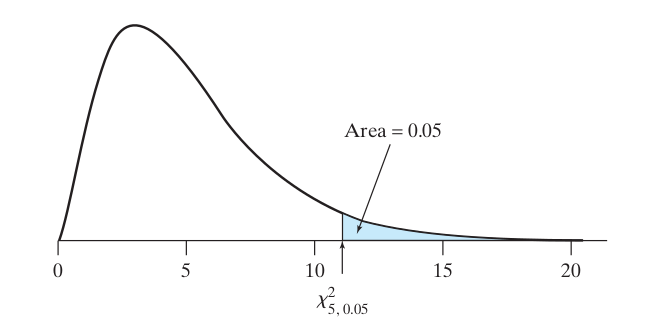
\includegraphics[width=0.6\textwidth]{fig9_4_4-chisq-histo}
  \end{center}

\end{frame}

\begin{frame}{Back to the example}

    Colorblindness in females:
    \begin{center}
        \begin{tabular}{r|rrr}
            & observed counts & expected counts & difference\\
            \hline 
            nonmutant & 850 & 840.9 & 9.1 \\ 
            carrier &  146 & 152.2 & -5.8 \\ 
            colorblind & 4 & 6.9 & 2.9  \\
        \end{tabular}
    \end{center}

    \vspace{2em}

    \begin{itemize}
      \item[$H_0$:] The prevalence of nonmutants, carriers, and colorblindness in European females is $(1-q)^2$, $2q(1-q)$, and $q^2$, with $q=0.083$.
      \item[$H_A$:] The prevalences in European females do not match those proportions.
    \end{itemize}

    \vspace{1em}

    \begin{align*}
        \chi^2_s &= \frac{9.1^2}{840.9} + \frac{5.8^2}{152.2} + \frac{2.9^2}{6.9} = 1.54 \\
        \df &= 3-1 = 2 .
      \end{align*}
      
      \vspace{1em}

      \alert{$P>0.2$.}

\end{frame}



%%%%%%
\begin{frame}{What do we conclude?}

    \begin{itemize}
      \item[$H_0$:] The prevalence of nonmutants, carriers, and colorblindness in European females is $(1-q)^2$, $2q(1-q)$, and $q^2$, with $q=0.083$.
      \item[$H_A$:] The prevalences in European females do not match those proportions.
    \end{itemize}
    \vspace{1em}

    \structure{Conclusion:} We do not have good statistical evidence that the proportions of European females that are colorblind, 
    or carry colorblindness alleles, differ from what we expect based on the male data ($P>0.2$, $\chi^2=1.54$, $\df=2$).



\end{frame}




% . . . 

\section<article>{Summary}
\section<presentation>*{Summary}

\begin{frame}{Summary}
  \begin{enumerate}
      \item The best estimator of the population frequency is not necessarily the sample frequency
      \item \ldots mostly because it gets tripped up for small frequencies.
      \item A good choice is \alert{Wilson's estimator} $\wt p$, that adds two imaginary observations of each type.
      \item The standard error of Wilson's estimator is $\sqrt{ \wt p (1-\wt p) / (n+4) }$,
      \item \ldots and confidence intervals for $\wt p$ are found using $z$ multipliers.
      \item Also: always think about what the results mean.
  \end{enumerate}
  and
  \begin{enumerate}
      \item We now have a good test statistic ($\chi^2_s$) to compare observed proportions
          to expected proportions in a sample.
      \item This test statistic has good theoretical properties.
      \item $\chi^2_s$ is equal to the sum of deviations of observed counts from expected counts, squared, and divided by the expected counts.
      \item The null distribution has one parameter, degrees of freedom, equal to the number of counts minus one.
  \end{enumerate}
\end{frame}

% homework
\begin{frame}{Homework}
  \begin{center}

  9.2.2

  \vspace{2em}

  9.2.9
  % \vspace{2em}
  % 9.2.10

  \vspace{2em}

  9.4.1
  % 9.4.6

  \end{center}
\end{frame}


\end{document}





